% !TeX program = xelatex
\documentclass[conference]{IEEEtran}
\IEEEoverridecommandlockouts
\usepackage{fontspec}
\setmainfont{LiberationSerif}[Path=fonts/,Extension=.ttf,UprightFont=*-Regular,BoldFont=*-Bold,ItalicFont=*-Italic,BoldItalicFont=*-BoldItalic]
\setsansfont{LiberationSans}[Path=fonts/,Extension=.ttf,UprightFont=*-Regular,BoldFont=*-Bold,ItalicFont=*-Italic,BoldItalicFont=*-BoldItalic]
\setmonofont{LiberationMono}[Path=fonts/,Extension=.ttf,UprightFont=*-Regular,BoldFont=*-Bold,ItalicFont=*-Italic,BoldItalicFont=*-BoldItalic,Scale=0.78]
\usepackage{amsmath,amssymb,graphicx,booktabs,array,cite,xurl,hyperref,microtype}
\usepackage{placeins}
\hypersetup{hidelinks,pdftitle={Auditing Shortcut Dependencies in DNS Tunneling: Residual Information across Models and Splits},pdfauthor={IAM302t Group 3}}
\newcommand{\code}[1]{\texttt{#1}}
\emergencystretch=1em
\newcommand{\RowRFFOne}{0.8864}
\newcommand{\RowRFAccuracy}{91.95}
\newcommand{\RFMean}{0.5250}
\newcommand{\RFSD}{0.4650}
\newcommand{\RFPooled}{0.6877}
\newcommand{\LRMean}{0.8043}
\newcommand{\LRSD}{0.1381}
\newcommand{\VectorRFFOne}{0.8863}
\newcommand{\ReferenceAccuracy}{91.90}
\newcommand{\ReferenceFOne}{0.8857}

\newcommand{\SeedOneFullMin}{0.8860}
\newcommand{\SeedOneFullMedian}{0.8863}
\newcommand{\SeedOneFullMax}{0.8865}
\newcommand{\SeedOneNoNameMin}{0.0000}
\newcommand{\SeedOneNoNameMedian}{0.0016}
\newcommand{\SeedOneNoNameMax}{0.0443}
\newcommand{\SeedTwoFullMin}{0.0004}
\newcommand{\SeedTwoFullMedian}{0.0004}
\newcommand{\SeedTwoFullMax}{0.0046}
\newcommand{\SeedTwoNoNameMin}{0.7759}
\newcommand{\SeedTwoNoNameMedian}{0.7759}
\newcommand{\SeedTwoNoNameMax}{0.7759}
\newcommand{\SeedThreeFullMin}{0.6773}
\newcommand{\SeedThreeFullMedian}{0.6879}
\newcommand{\SeedThreeFullMax}{0.6883}
\newcommand{\SeedThreeNoNameMin}{0.3340}
\newcommand{\SeedThreeNoNameMedian}{0.3340}
\newcommand{\SeedThreeNoNameMax}{0.3340}

\begin{document}
\title{Auditing Shortcut Dependencies in DNS Tunneling:\\Supplemental Audit Record}
\author{\IEEEauthorblockN{Mai Chí Thành \quad Đỗ Quang Thuận\\Nguyễn Lê Quốc Bảo \quad Đặng Nguyễn Phương Thảo}
\IEEEauthorblockA{Group 3, IA2007, FPT University\\VM-verified revision of November 4, 2026}}
\maketitle
\begin{abstract}
This supplement records the complete frozen-split results, five-seed RF experiment, model inventories, laboratory controls, RF path checks, and CTU provenance behind the focused main paper. Original VM evidence and subsequent diagnostic archives are retained. Findings can be checked from saved predictions without retraining.
\end{abstract}

\section{Reading Map and Evidence Files}
The main paper contains four displays: the common audit framework, compact CIC controls, the RF failure/input-sensitivity figure, and the CTU representation figure. This supplement carries detailed numerical inventories. The source archive contains the CSV and NPZ evidence at full precision; displayed tables round only for readability.

\begin{itemize}
\item \code{results/*\_results.csv}: all original CIC metrics; \code{results/predictions/}: the 50 primary LR/RF row-prediction arrays.
\item \code{splits/frozen\_splits.npz} and \code{metadata.json}: immutable indices and dataset/split SHA-256 bindings.
\item \code{results/revision\_v2/}: eight verified mechanism refits, cohort score sensitivity, four CTU controls, feature profiles, and exact per-tree paths.
\item \code{results/paper\_rf\_seeds/}: all 30 seed cases, row-level scores, fixed plan, paired comparisons, and independent verification receipt.
\item \code{lab/results/}: missing-value, graph-ablation, transaction, and false-positive audits.
\item \code{docs/CTU\_PIPELINE\_TRACE.md}: pinned source inspection and the distinction between exposure and score reproduction.
\end{itemize}

The term ``domain removed'' in historical filenames refers to deletion of 14 numeric name statistics. It does not remove all information associated with domains. The \code{sld} field is a grouping variable, absent from the 43 primary inputs. A separate 41-field reference control does include supplied categorical columns and must not be conflated with that primary pipeline.

\section{Frozen CIC Partitions and Input Inventory}
\begin{table*}[t]
\caption{All frozen CIC partitions. Shared vectors counts distinct complete 41-field nonlabel vectors, whereas repeated test-row counts are measured separately. GROUP folds hold out exact coarse tokens, not validated registered domains.}
\centering\footnotesize
\begin{tabular}{@{}lrrrrrr@{}}
\toprule
Protocol & Train & Test & Test benign & Test attack & Shared SLD & Shared vectors\\\midrule
ROW & 159,629 & 68,413 & 46,804 & 21,609 & 15,918 & 1,272\\
GROUP 1 & 152,028 & 76,014 & 35,453 & 40,561 & 0 & 0\\
GROUP 2 & 152,028 & 76,014 & 49,807 & 26,207 & 0 & 0\\
GROUP 3 & 152,028 & 76,014 & 70,754 & 5,260 & 0 & 0\\
EXACT VECTOR GROUP & 162,240 & 65,802 & 46,256 & 19,546 & 15,853 & 0\\
\bottomrule
\end{tabular}

\end{table*}
The unchanged CSV SHA-256 is \nolinkurl{62ec5d632c9e665851c551487d6d1e2afbc7f8f55b62cac4649999dadafc89de}; the saved split archive SHA-256 is \nolinkurl{a48ccdaf3995390f3af063cb107429738149ee546dda24d14804c30a3d2641d5}. Neither the new probes nor the report build regenerates these indices.

The 14 supplied name-statistic inputs are \code{FQDN\_count}, \code{subdomain\_length}, \code{upper}, \code{lower}, \code{numeric}, \code{entropy}, \code{special}, \code{labels}, \code{labels\_max}, \code{labels\_average}, \code{len}, \code{subdomain}, \code{rr\_name\_entropy}, and \code{rr\_name\_length}. Explicit type inputs consist of a frequency and an indicator for each of A, AAAA, NS, CNAME, SOA, NULL, PTR, HINFO, MX, TXT, SRV, and OPT. The five remaining inputs are \code{rr\_count}, \code{a\_records}, \code{ttl\_mean}, \code{ttl\_variance}, and \code{distinct\_ns}.

RF uses zero fill with empty features retained, 100 trees, maximum depth 16, minimum leaf size two, seed 42, and two jobs. LR removes candidate columns with fewer than ten numeric training observations or only one distinct training value; then zero fill, standard scaling, and balanced logistic regression use $C=0.5$, seed 42, and 2,000 maximum iterations. All preprocessing is fitted on the relevant training indices.

Six conditions are retrained: FULL; NO-QTYPE; NO-DOMAIN; NO-BOTH; NO-QTYPE-TTL; and NO-BOTH-TTL. QTYPE removes 24 direct type columns; DOMAIN removes the 14 name statistics; TTL removes mean and variance TTL. FULL also uses exact-vector exclusion. The complete LR/RF CSVs include TN, FP, FN, TP, precision, recall, accuracy, F1, and FPR for every case.

\begin{table*}[t]
\caption{Complete CIC feature ablation. G1--G3 are all coarse-token folds. SD is the sample SD across folds, not a confidence interval; pooled F1 uses summed fold confusion counts. ``Neither'' removes explicit type and name statistics; ``/TTL'' additionally removes TTL.}
\centering\footnotesize
\begin{tabular}{@{}llrrrrrrrr@{}}
\toprule
Model & Feature set & Row F1 & Row FPR\% & G1 F1 & G2 F1 & G3 F1 & Mean F1 & SD & Pooled F1\\\midrule
LR & Full & 0.8816 & 11.53 & 0.8827 & 0.8853 & 0.6449 & 0.8043 & 0.1381 & 0.8689\\
LR & No type & 0.8567 & 13.10 & 0.7923 & 0.8578 & 0.6644 & 0.7715 & 0.0984 & 0.8056\\
LR & No domain & 0.7546 & 29.23 & 0.8817 & 0.7801 & 0.3339 & 0.6652 & 0.2914 & 0.7555\\
LR & Neither & 0.7419 & 27.65 & 0.8632 & 0.7667 & 0.3339 & 0.6546 & 0.2819 & 0.7429\\
LR & No type/TTL & 0.8394 & 13.79 & 0.7948 & 0.8530 & 0.6636 & 0.7705 & 0.0970 & 0.8054\\
LR & Neither/TTL & 0.6026 & 60.86 & 0.7887 & 0.6332 & 0.1968 & 0.5395 & 0.3069 & 0.6025\\
RF & Full & 0.8864 & 11.55 & 0.8862 & 0.0004 & 0.6883 & 0.5250 & 0.4650 & 0.6877\\
RF & No type & 0.8869 & 11.56 & 0.8866 & 0.0003 & 0.6800 & 0.5223 & 0.4637 & 0.6875\\
RF & No domain & 0.7544 & 28.97 & 0.0016 & 0.7759 & 0.3340 & 0.3705 & 0.3885 & 0.4470\\
RF & Neither & 0.7528 & 29.09 & 0.0000 & 0.7759 & 0.3339 & 0.3699 & 0.3892 & 0.4471\\
RF & No type/TTL & 0.8861 & 11.61 & 0.8779 & 0.0002 & 0.6645 & 0.5142 & 0.4578 & 0.6797\\
RF & Neither/TTL & 0.0000 & 0.00 & 0.0000 & 0.0000 & 0.1968 & 0.0656 & 0.1136 & 0.0875\\
\bottomrule
\end{tabular}

\end{table*}

\begin{figure*}[t]
\centering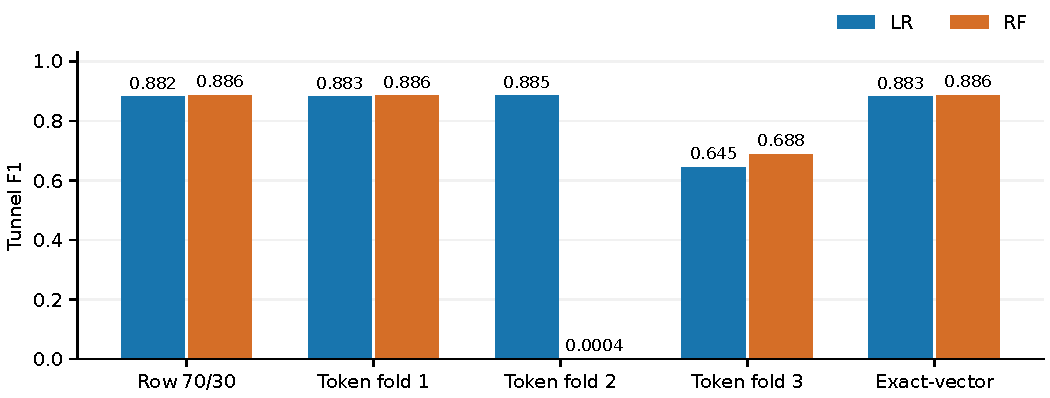
\includegraphics[width=.94\textwidth]{figures/fixed_split_models.pdf}
\caption{All FULL-model partitions. The coarse-token diagnostic has a different population meaning from the ROW and exact-vector splits. No fold is selected by score.}
\end{figure*}

\section{Identity and Residual-Type Controls}
\begin{table}[!htbp]
\caption{Record-equivalence inventory for the unchanged CIC copy. The supplied 41-field vector is not identical to the 43 numeric model-input vector.}
\centering\footnotesize
\begin{tabular}{@{}p{4.55cm}r@{}}
\toprule
Measurement & Count\\\midrule
Rows & 228,042\\
Duplicate complete rows beyond first & 86,866\\
Distinct nonlabel vectors & 140,176\\
Vectors carrying both labels & 1,000\\
Rows in those conflicting vectors & 87,524\\
Row-test vectors also observed in train (rows) & 26,807\\
\bottomrule
\end{tabular}

\end{table}
A complete-row duplicate includes the label and all supplied fields. A nonlabel-equivalent group ignores only the label. Its opposite labels can indicate unresolved ambiguity at the feature resolution; they do not identify incorrect packet ground truth by themselves. Hash-based conflicting candidates were checked against exact cell equality. The empirical minimum error of a deterministic function of all 41 supplied fields, over the entire labeled CSV, is 17,541 rows. That descriptive all-row floor is not a bound on a separately sampled test subset.

Token \code{192} contains 74,740 rows (34,179 benign; 40,561 attack); \code{224} contains 48,357 (22,159 benign; 26,198 attack). Every GROUP-1 test attack has token \code{192}. GROUP 2 contains 26,207 attacks, of which 26,198 have token \code{224}. These raw normalized strings are not a hash encoding invented by this audit. They do not provide enough information to reconstruct full query names or validate Public Suffix List parsing.

\begin{table}[!htbp]
\caption{Held-out accuracy (\%) for auxiliary PTR-versus-other prediction using a depth-three tree. OTHER consists of the five response measurements and includes TTL.}
\centering\footnotesize
\begin{tabular}{@{}lrrrr@{}}
\toprule
Inputs for PTR classifier & Row & G1 & G2 & G3\\\midrule
TTL only & 98.14 & 97.78 & 98.18 & 98.79\\
Other fields & 98.14 & 97.78 & 98.18 & 98.79\\
Other without TTL & 75.23 & 81.02 & 75.90 & 68.71\\
\bottomrule
\end{tabular}

\end{table}
The all-row post-hoc rule ``mean TTL in $\{1,255\}$'' identifies PTR with 98.25\% accuracy. Its rule selection has no independent holdout. The depth-three train/test experiment is the appropriate held-out evidence that type information persists. It predicts PTR membership, not the benign/attack label.

\begin{table}[!htbp]
\caption{Reference-inventory single-stage RF on the same ROW split. This control uses all 41 supplied nonlabel fields before encoding; it is distinct from the primary 43-input baseline.}
\centering\footnotesize
\begin{tabular}{@{}lrrrr@{}}
\toprule
Feature set & Inputs & Accuracy\% & F1 & FPR\%\\\midrule
Full & 41 & 91.90 & 0.8857 & 11.52\\
No type & 28 & 91.96 & 0.8867 & 11.56\\
No domain & 25 & 79.75 & 0.7545 & 28.91\\
Neither & 12 & 79.69 & 0.7551 & 29.31\\
\bottomrule
\end{tabular}

\end{table}
The reference control averages TTL lists, fits ordinal categorical encoding on training rows (unknown value $-1$), and uses 100 RF trees without a depth cap and with minimum leaf size one. It obtains FULL accuracy 91.90\% and F1=0.8857. The published CIC hybrid's reported 99.97\% score involves stateless classification, suspicious-window gating, and stateful re-analysis. Without the paired timestamped stateless sequence and gating trace, subtracting these scores would not measure shortcut inflation in the original system. The protocol-alignment document retains the required inputs and distinctions.

\section{RF Mechanism: Prediction Checks and Paths}
All eight refits (RF/LR, GROUP 1/2, FULL/NO-DOMAIN) reproduce the saved VM predictions row for row. A negative control replacing every \code{sld} value while holding split indices fixed leaves all model inputs unchanged. This rules out a literal token condition in the primary RF; it does not rule out numeric proxies correlated with the token populations.

\begin{table}[!htbp]
\caption{Largest absolute path-score contributions for one common GROUP-2 RF false-negative input vector (original CSV row index 11; repeated 2,192 times among false negatives). Contributions average visited child-minus-parent positive proportions across trees.}
\centering\footnotesize
\begin{tabular}{@{}lr@{}}
\toprule
RF input & Mean path-score contribution\\\midrule
entropy & -0.1067\\
len & -0.0855\\
special & +0.0831\\
FQDN\_count & -0.0729\\
raw\_type\_A & +0.0586\\
subdomain\_length & -0.0558\\
ttl\_mean & +0.0418\\
raw\_type\_PTR & +0.0408\\
\bottomrule
\end{tabular}

\end{table}
For this vector, the mean root positive proportion is 0.301567. Adding all 43 feature contributions gives 0.344529, equal to RF's direct positive-class probability within $10^{-10}$. The selected terms do not sum to that score without the remaining terms. Full paths, thresholds, and per-tree leaf probabilities are in \code{mechanism.json}; the decomposition depends on traversal order and is not a Shapley-value explanation.

In the first tree, \code{labels\_average}$\leq3.9167$ and \code{raw\_type\_PTR}$>0.5$ initially raise the positive proportion. The branch \code{FQDN\_count}$\leq24$ then lowers it by 0.6562; subsequent entropy/label splits end at a zero-positive leaf. Across trees, commonly traversed downward name splits include \code{subdomain\_length}$\leq7.5$, \code{FQDN\_count}$\leq24.5$, and \code{len}$\leq11.5$. These describe actual numeric thresholds, rather than a rule on an absent textual field.

\begin{table}[!htbp]
\caption{Median GROUP-2 positive-class scores under the fixed input substitution. The replacement is applied identically to every test row using training-attack medians; summaries use actual classes only after scoring.}
\centering\footnotesize
\begin{tabular}{@{}llrr@{}}
\toprule
Model & Actual class & Observed $p$ & Prototype $p$\\\midrule
RF & Benign & 0.0047 & 0.0252\\
RF & Attack & 0.3326 & 0.8056\\
LR & Benign & 0.0002 & 0.1171\\
LR & Attack & 0.7859 & 0.9170\\
\bottomrule
\end{tabular}

\end{table}
The prototype replaces only the 14 name statistics. For the GROUP-2 training attacks, notable medians are \code{FQDN\_count}=27, \code{subdomain\_length}=10, entropy=2.674526, and \code{len}=14. The remaining type and response inputs stay at their observed values. The probe increases the fraction of positive predictions among attack rows from 0.019\% to 99.069\% for RF, but also from 0.004\% to 28.904\% among benign rows. LR's attack fraction changes from 99.054\% to 99.065\%, while its benign fraction increases from 13.008\% to 28.906\%. These are sensitivities of fixed models to artificial inputs, not new detector operating points or deployment scores.

\FloatBarrier
\section{RF Stability across Five Fixed Forest Seeds}
Before the additional run, we fixed seeds 42, 0, 1, 7, and 2026, all three frozen GROUP folds, and FULL/NO\_DOMAIN: 30 cases. This was a recorded analysis plan, not a public preregistration. Only the forest random seed changes; preprocessing, 100 trees, maximum depth 16, minimum leaf size two, and default prediction remain fixed. No result selects a seed or threshold. The plan and its canonical SHA-256 are retained with the execution log.

\begin{table}[!htbp]
\caption{RF F1 across all five forest seeds. Minima, medians, and maxima describe variation on the same frozen test rows; they are not confidence intervals from independent traffic samples.}
\label{tab:seeds_summary}
\centering\footnotesize
\begin{tabular}{@{}llrrr@{}}
\toprule
Fold & Inputs & Min F1 & Median F1 & Max F1\\\midrule
G1 & Full & 0.886002 & 0.886325 & 0.886487\\
G1 & No name & 0.000000 & 0.001576 & 0.044275\\
G2 & Full & 0.000381 & 0.000381 & 0.004641\\
G2 & No name & 0.775907 & 0.775907 & 0.775950\\
G3 & Full & 0.677327 & 0.687893 & 0.688258\\
G3 & No name & 0.333996 & 0.333996 & 0.334007\\
\bottomrule
\end{tabular}

\end{table}
\begin{table*}[t]
\caption{Every RF seed case, paired within fold and seed. ``No name'' removes 14 numeric name statistics. All other model settings and indices are fixed; each row contains two fits. Full confusion counts, scores, and indices are saved.}
\label{tab:seeds_all}
\centering\footnotesize
\begin{tabular}{@{}lrrrrrrr@{}}
\toprule
Fold & Seed & Full F1 & No-name F1 & Full FP & No-name FP & Full TP & No-name TP\\\midrule
G1 & 42 & 0.886224 & 0.001576 & 9,956 & 4 & 40,196 & 32\\
G1 & 0 & 0.886002 & 0.001576 & 9,951 & 4 & 40,174 & 32\\
G1 & 1 & 0.886378 & 0.001576 & 9,959 & 4 & 40,211 & 32\\
G1 & 7 & 0.886487 & 0.000000 & 9,963 & 0 & 40,223 & 0\\
G1 & 2026 & 0.886325 & 0.044275 & 9,962 & 210 & 40,209 & 923\\
G2 & 42 & 0.000381 & 0.775907 & 2 & 14,002 & 5 & 25,487\\
G2 & 0 & 0.000381 & 0.775907 & 2 & 14,002 & 5 & 25,487\\
G2 & 1 & 0.004641 & 0.775907 & 17 & 14,002 & 61 & 25,487\\
G2 & 7 & 0.000381 & 0.775907 & 2 & 14,002 & 5 & 25,487\\
G2 & 2026 & 0.000381 & 0.775950 & 2 & 14,011 & 5 & 25,495\\
G3 & 42 & 0.688258 & 0.334007 & 795 & 20,707 & 3,177 & 5,206\\
G3 & 0 & 0.687906 & 0.333996 & 794 & 20,708 & 3,174 & 5,206\\
G3 & 1 & 0.687893 & 0.334007 & 798 & 20,707 & 3,176 & 5,206\\
G3 & 7 & 0.677327 & 0.333996 & 778 & 20,708 & 3,092 & 5,206\\
G3 & 2026 & 0.686910 & 0.333996 & 794 & 20,708 & 3,167 & 5,206\\
\bottomrule
\end{tabular}

\end{table*}
\begin{figure*}[t]
\centering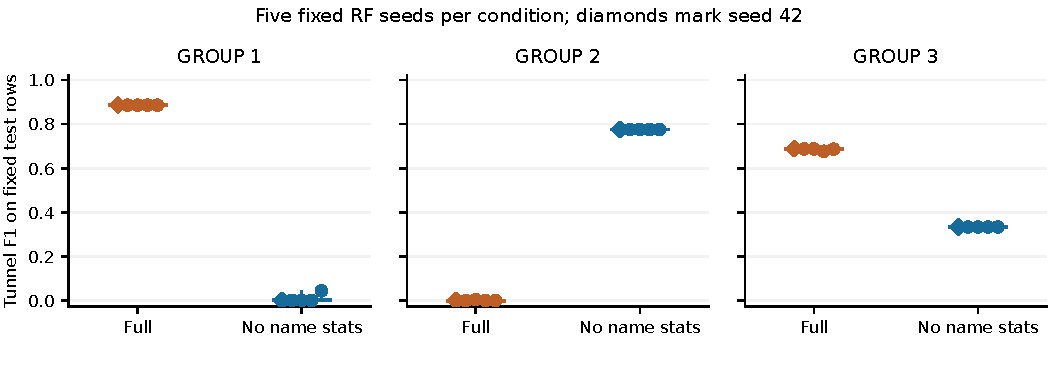
\includegraphics[width=.94\textwidth]{figures/rf_seed_stability.pdf}
\caption{All five seed F1 values per RF condition; diamonds mark the reference seed 42, horizontal lines mark medians, and vertical segments span min--max. Small deterministic horizontal offsets separate coincident points and do not encode a second variable. The ablation direction is the same at every seed on each fold.}
\label{fig:seed_stability}
\end{figure*}

All six seed-42 predicted-label arrays match the original baseline exactly. Independently recomputing confusion counts from CSV labels and NPZ predictions reproduces all 30 cases, six summaries, and 15 paired differences. The source, dataset, split, and VM environment agree with the fixed plan and previous receipt. The original received archive is preserved unchanged.

GROUP-2 FULL detects only 5--61 of 26,207 attacks across seeds (F1 \SeedTwoFullMin--\SeedTwoFullMax); removing name statistics yields F1 approximately 0.7759. GROUP-1 FULL stays at \SeedOneFullMin--\SeedOneFullMax, while no-name F1 ranges from zero (seed 7) to 0.044275 (seed 2026). GROUP-3 FULL ranges from \SeedThreeFullMin\ to \SeedThreeFullMax; its no-name F1 stays near 0.3340. FULL-minus-no-name F1 is positive on GROUP 1/3 and negative on GROUP 2 at every paired seed. These results support persistence of the fold-specific response under forest randomness. They add neither new traffic populations nor a validated domain/family holdout.

\FloatBarrier
\section{CTU Provenance, Representations, and Controls}
\begin{table}[!htbp]
\caption{Binary CTU structure after trim/lowercase/trailing-root-dot canonicalization. Class 1 here means the retained tunnel label, remapped from original multiclass label 2.}
\centering\footnotesize
\begin{tabular}{@{}llrrrr@{}}
\toprule
Split & Class & Rows & No dots & 1 dot & $\geq2$ dots\\\midrule
TRAIN & Benign & 944,106 & 944,106 & 0 & 0\\
TRAIN & Tunnel & 6,441 & 6,441 & 0 & 0\\
TEST & Benign & 236,072 & 47 & 208,314 & 27,711\\
TEST & Tunnel & 1,559 & 0 & 0 & 1,559\\
\bottomrule
\end{tabular}

\end{table}
\begin{table}[!htbp]
\caption{Original multiclass raw-string counts, before binary filtering or canonicalization. Original labels 0/1/2 denote benign/DGA/tunnel. The last column checks dots surviving a first-45-character truncation.}
\centering\footnotesize
\begin{tabular}{@{}llrrr@{}}
\toprule
Split & Class & Rows & Any dot & Dot in first 45\\\midrule
Train & Benign & 944,106 & 0 & 0\\
Train & DGA & 1,532,263 & 0 & 0\\
Train & Tunnel & 6,441 & 0 & 0\\
Test & Benign & 236,072 & 236,027 & 236,027\\
Test & DGA & 383,072 & 383,071 & 383,071\\
Test & Tunnel & 1,559 & 1,559 & 1,257\\
\bottomrule
\end{tabular}

\end{table}
Both files are from Zenodo record 6508640. Publisher MD5 values are \code{c30a49c6f362e0c2dffe3881504a6825} (train) and \code{ce52df239c4245ffaa15c642b8b0b625} (test). Saved preparation metadata records original SHA-256, binary SHA-256, source URLs, original counts, and unchanged-domain class filtering. Fresh original downloads match both publisher MD5 and saved SHA-256. The two extra dotted raw benign test strings lose their trailing dot under canonicalization, explaining 236,027 raw versus 236,025 canonical dotted benign strings.

All 950,547 binary training strings satisfy length=max-label-length=mean-label-length. Only 47 binary test strings satisfy that identity. These deterministic constraints locate a change in the joint lexical representation, not merely a shift in the mean value of one feature.

\begin{table}[!htbp]
\caption{Original CTU lexical controls. Training is unchanged; only test representation differs. LENGTH uses a threshold selected from seven candidates by training F1, selecting 30.}
\centering\footnotesize
\begin{tabular}{@{}llrrrr@{}}
\toprule
Model & Test input & FP & TP & F1 & FPR\%\\\midrule
LENGTH & Full & 1,516 & 1,475 & 0.6484 & 0.64\\
LENGTH & First label & 245 & 820 & 0.6250 & 0.10\\
LR8 & Full & 4,739 & 906 & 0.2515 & 2.01\\
LR8 & First label & 12,039 & 1,049 & 0.1432 & 5.10\\
LR4 & Full & 29,187 & 1,559 & 0.0965 & 12.36\\
LR4 & First label & 19,524 & 1,122 & 0.1011 & 8.27\\
\bottomrule
\end{tabular}

\end{table}
The eight lexical measurements are total length, dot count, maximum/mean label length, digit/hyphen fractions, character entropy, and unique-character fraction. LR4 keeps only the final four. Standardization and LR ($C=0.5$, balanced, seed 42, 2,000 iterations) are trained on the original binary training subset. First-label extraction is a lossy sensitivity probe, not registrable-domain parsing or a validated repair. Last-label and last-two-label rules each predict every test row as benign, giving both zero recall and zero FPR.

\begin{table}[!htbp]
\caption{Additional constant-dot negative control. LR7 omits only dot count. In each representation its entire predicted-label array equals LR8's array; the fitted LR8 dot-count coefficient is zero.}
\centering\footnotesize
\begin{tabular}{@{}llrrrr@{}}
\toprule
Inputs & Test string & FP & TP & F1 & FPR\%\\\midrule
LR8 & Full & 4,739 & 906 & 0.2515 & 2.01\\
LR8 & First label & 12,039 & 1,049 & 0.1432 & 5.10\\
LR7\_NO\_DOTS & Full & 4,739 & 906 & 0.2515 & 2.01\\
LR7\_NO\_DOTS & First label & 12,039 & 1,049 & 0.1432 & 5.10\\
\bottomrule
\end{tabular}

\end{table}
The no-dot control is distinct from deleting suffixes. Removing a constant training feature cannot resolve inconsistent total/label lengths, character distributions, or a change in the strings presented to a character-level model.

\subsection{Trace to Published Work}
The 2019 MC-CNN paper's Table 3 has test supports 236,072 normal, 383,072 DGA, and 1,559 tunnel, matching the released test files \cite{ctupaper}. This is a concrete release-to-publication consistency check; it does not identify the exact original train/test preprocessing commands or checkpoint. The paper's prose also describes a 70/30 split, while the released class counts are approximately 80/20; the support match should not be promoted to a complete run reconstruction.

The author-associated deepseq repository is pinned at commit \code{769e3466f90173b663aa1fe3008e7a70295fbdfd}. The inspected files are \code{preprocess.R}, \code{deepseq\_classifier.R}, \code{config.R}, and \code{model\_mc\_cnn\_asai.R}. Their hashes and relevant line locations are recorded in the source-trace metadata. The functions build character sequences with end padding/truncation, the command-line default maximum length is 45, and an external test file goes through the same dataset builder. The inspected preprocessing does not remove suffixes.

Under the corresponding first-45-character exposure check, the raw release still has dots in 236,027 normal, 383,071 DGA, and 1,257 tunnel test strings; training has none. This is an input exposure measurement, not an execution of that R/neural pipeline. The inspected configuration has alternative vocabulary/data settings; neither the exact 2019 vocabulary/configuration nor its checkpoint is established. Consequently, the audit identifies a serious artifact that subsequent evaluations should check, without declaring every published CTU score invalid. The 2020 follow-up introduces a different five-tool dataset \cite{palau2020}; a release-specific finding must not be transferred to it without verifying that dataset's files.

\FloatBarrier
\section{Laboratory and One-Sided Capture Details}
\begin{table}[!htbp]
\caption{LAB zero/median replay on all 90 evaluation groups. Full CSV outputs additionally include missingness indicators and restricted-population diagnostics.}
\centering\footnotesize
\begin{tabular}{@{}llrrrrr@{}}
\toprule
Features & Imputer & TN & FP & FN & TP & F1\\\midrule
Control & Zero & 77 & 0 & 0 & 13 & 1.0000\\
Control & Median & 77 & 0 & 0 & 13 & 1.0000\\
POINT & Zero & 71 & 6 & 0 & 13 & 0.8125\\
POINT & Median & 71 & 6 & 0 & 13 & 0.8125\\
GRAPH & Zero & 77 & 0 & 0 & 13 & 1.0000\\
GRAPH & Median & 77 & 0 & 0 & 13 & 1.0000\\
HYBRID & Zero & 71 & 6 & 0 & 13 & 0.8125\\
HYBRID & Median & 73 & 4 & 0 & 13 & 0.8667\\
\bottomrule
\end{tabular}

\end{table}
The ordinary client is \code{192.168.10.10}; the iodine client is \code{192.168.10.20}. The prior pilot has 15 training groups (eight normal/seven tunnel). The evaluated capture has 3,542 queries (1,393 normal/2,149 tunnel), yielding 77 normal and 13 tunnel 300-s groups. All 13 tunnel groups originate from one approximately 61-min session, so they are not 13 independently generated attack scenarios.

POINT uses name length/entropy, subdomain entropy, mean interarrival, its coefficient of variation, and SERVFAIL ratio. GRAPH uses distinct names/subdomains, singleton ratio, name-frequency entropy, client--domain degree, domain--client degree, domain--answer-IP degree, and client--domain query share. HYBRID concatenates both families. All use balanced LR, $C=0.5$, and train-fitted scaling.

\begin{table}[!htbp]
\caption{Graph-family deletions in the observed laboratory scenario. The complete CSV also includes minimal-diversity and point/hybrid controls.}
\centering\footnotesize
\begin{tabular}{@{}lrrr@{}}
\toprule
Removed graph input & Kept & FP & F1\\\midrule
None & 8 & 0 & 1.0000\\
Client--domain degree & 7 & 0 & 1.0000\\
Domain query share & 7 & 0 & 1.0000\\
Domain--answer-IP degree & 7 & 5 & 0.8387\\
All three proxies & 5 & 0 & 1.0000\\
Three proxies + QNAME count & 4 & 0 & 1.0000\\
\bottomrule
\end{tabular}

\end{table}
There are 3,541 matched transactions: normal has 1,279 NOERROR and 114 SERVFAIL; the tunnel has 2,148 NOERROR and one unmatched query. The 96 latencies over ten seconds are all normal. Five POINT/HYBRID false positives are single-query \code{ubuntu.com} groups; the sixth is a two-query \code{fwupd.org} group. All-column missing indicators are constructed explicitly but have no training variation, so their fitted coefficients cannot learn a missingness effect. Restricting to groups with at least two queries changes the evaluated population and leaves 85 test groups.

Source, zone, NULL-type, distinct-name-count, and name-frequency-entropy post-hoc rules each perfectly separate this lab setting. Jointly deleting three suspected graph proxies still leaves perfect classification, because remaining features also separate the same scenario. These findings motivate the residual-information audit rather than establish an advantage of graph modeling in independent deployments.

The selected Korving BIND9/iodine CNAME--Base64 PCAP has 26,761 observed DNS queries, all CNAME. Of these, 13,373 are client-side and 13,388 forwarder-side, representing collection legs of one attack scenario. No independently labeled benign counterpart is present, so no binary F1 is reported for this source.

\FloatBarrier
\newpage
\section{Verification and Reproduction}
Run \code{source/verify\_revision.py} without retraining to recompute the 50 core confusion matrices, check eight prediction-identical refits, verify saved cohort summaries, compare four CTU controls, and check dataset/split bindings and the RF path sum. Run \code{source/verify\_rf\_seed\_check.py} for all 30 seed cases, six summaries, 15 paired differences, six baseline matches, and the plan/archive bindings. Original VM logs and receipts remain unchanged.

The additional controls were rerun on the VM with Python 3.12.16 and all 18 packages matching the lock file. Against the earlier Python 3.12.14 run, all predicted labels agree. The largest LR score difference is 0.004524 on observed inputs and 0.005063 under the artificial cohort substitution; its cause was not isolated. RF refit scores match exactly. Current tables use VM scores; the original reference arrays and comparison receipt are preserved. The source guide covers downloads, refits, and compilation with frozen indices.

\paragraph{Code availability}
Source, frozen splits, and reproduction instructions are available at \url{https://github.com/QuangApollo/iam302t-dns-shortcut-audit}. The LMS submission includes complete row-level predictions and original VM evidence. Checksum-pinned scripts retrieve the public datasets.


\paragraph{AI use and authorship}
The main paper's AI disclosure applies here. Authors remain responsible for review; scripts and saved outputs expose the numerical basis.

\begin{thebibliography}{3}
\bibitem{ctupaper} F. Palau, C. Catania, J. Guerra, S. Garcia, and M. Rigaki, ``Detecting DNS threats: A deep learning model to rule them all,'' in \emph{XX Simposio Argentino de Inteligencia Artificial, JAIIO 48}, pp. 90--101, 2019. \url{https://sedici.unlp.edu.ar/handle/10915/87859}.
\bibitem{palau2020} F. Palau et al., ``DNS tunneling: A deep learning based lexicographical detection approach,'' arXiv:2006.06122v2, 2020, doi:10.48550/arXiv.2006.06122.
\end{thebibliography}
\end{document}
